\begin{enumerate}[label=\thechapter.\arabic*,ref=\thechapter.\theenumi]
\item
For the circuit given below, choose the angular frequency $ \omega_0$ at which voltage across capacitor has maximum amplitude?
\begin{figure}[h!]
    \includegraphics[width = 0.5\columnwidth]{2023/BM/16/figs/c_fig1.pdf}
    \caption{circuit }
    \centering
    \label{fig: bm_16_fig_1}
\end{figure}
\begin{enumerate}
    \item[(A)] 1000
    \item[(B)] 100
    \item[(C)] 1
    \item[(D)] 0   
\end{enumerate}
\hfill(GATE BM 2023 Question 16)\\

\solution
\input{2023/BM/16/asnmt3.tex}
\newpage
\item
In the following circuit, the switch S is open for $t < 0$ and closed for $t \ge 0$.
What is the steady state voltage (in Volts) across the capacitor when the switch is closed?
\begin{figure}[h!]
    \includegraphics[width = 0.7\columnwidth]{2023/BM/30/figs/c_fig1.pdf}
    \caption{circuit }
    \centering
    \label{fig:bm_30_fig_1}
\end{figure}
\hfill(GATE BM 2023 Question 30) \\
\solution
\iffalse
\let\negmedspace\undefined
\let\negthickspace\undefined
\documentclass[journal,12pt,twocolumn]{IEEEtran}
\usepackage{cite}
\usepackage{amsmath,amssymb,amsfonts,amsthm}
\usepackage{algorithmic}
\usepackage{graphicx}
\usepackage{textcomp}
\usepackage{xcolor}
\usepackage{txfonts}
\usepackage{listings}
\usepackage{enumitem}
\usepackage{mathtools}
\usepackage{gensymb}
\usepackage{comment}
\usepackage[breaklinks=true]{hyperref}
\usepackage{tkz-euclide}
\usepackage{listings}
\usepackage{gvv}
\def\inputGnumericTable{}
\usepackage[latin1]{inputenc}
\usepackage{color}
\usepackage{array}
\usepackage{longtable}
\usepackage{calc}
\usepackage{multirow}
\usepackage{hhline}
\usepackage{ifthen}
\usepackage{lscape}

\newtheorem{theorem}{Theorem}[section]
\newtheorem{problem}{Problem}
\newtheorem{proposition}{Proposition}[section]
\newtheorem{lemma}{Lemma}[section]
\newtheorem{corollary}[theorem]{Corollary}
\newtheorem{example}{Example}[section]
\newtheorem{definition}[problem]{Definition}
\newcommand{\BEQA}{\begin{eqnarray}}
\newcommand{\EEQA}{\end{eqnarray}}
\newcommand{\define}{\stackrel{\triangle}{=}}
\theoremstyle{remark}
\newtheorem{rem}{Remark}
\begin{document}

\bibliographystyle{IEEEtran}
\vspace{3cm}

\title{GATE 2023 BM 30}
\author{EE23BTECH11007 - Aneesh Kadiyala$^{*}$% <-this % stops a space
}
\maketitle
\newpage
\bigskip

\renewcommand{\thefigure}{\theenumi}
\renewcommand{\thetable}{\theenumi}

\vspace{3cm}
\textbf{Question:} In the following circuit, the switch S is open for $t < 0$ and closed for $t \ge 0$.
What is the steady state voltage (in Volts) across the capacitor when the switch is closed?
\begin{figure}[h!]
    \centering
    \includegraphics[width = \columnwidth]{2023/BM/30/figs/c_fig1.pdf}
\end{figure}
\\
\solution
\\
\fi
\begin{figure}[h!]
    \centering
    \includegraphics[width=\columnwidth]{2023/BM/30/figs/c_fig3.pdf}
\end{figure}
\\
In steady state, no current flows through the capacitor.
\begin{align}
I_2 &= 0 \\
V_c &= \brak{7\text{k}\ohm}I_1 \\
&= \brak{7\text{k}\ohm}I \\
&= \brak{7\text{k}\ohm}\frac{10\text{V}}{10\text{k}\ohm} \\
\implies V_c &= 7\text{V}
\end{align}
In s-domain:
\begin{figure}[h!]
    \centering
    \includegraphics[width=\columnwidth]{2023/BM/30/figs/c_fig2.pdf}
\end{figure}
\begin{align}
\implies I\brak{s} &= \frac{\frac{10}{s}\text{V}}{3\text{k}\ohm + \frac{(7\text{k}\ohm)(10\text{k}\ohm + \frac{1}{sC})}{17\text{k}\ohm + \frac{1}{sC}}} \\
I &= I_1 + I_2 \\
I_1\brak{7\text{k}\ohm} &= I_2\brak{10\text{k}\ohm + \frac{1}{sC}} \\
I_2\brak{s} &= \frac{7\text{k}\ohm}{17\text{k}\ohm + \frac{1}{sC}}I\brak{s} \\
%&= \frac{\frac{70000}{s}}{121 * 10^6 + \frac{10000}{sC}} \\
%&= \frac{\frac{7}{s}}{121 * 10^2 + \frac{1}{sC}} \\
\implies I_2\brak{s} &= \frac{7\brak{10^{-5}}}{0.121s + 1} \\
V_c\brak{s} &= I_2\brak{s}\frac{1}{sC} \\
&= \frac{7}{s\brak{0.121s + 1}} \\
%&= 7\brak{\frac{\frac{1}{0.121}}{s\brak{s + \frac{1}{0.121}}}} \\
&= 7\brak{\frac{1}{s} - \frac{1}{s + \frac{1}{0.121}}}
\end{align}
Taking inverse Laplace transform:
\begin{align}
V_c\brak{t} &= 7u\brak{t}\brak{1 - e^{-\frac{t}{-0.121}}} \label{eq:2023BM30}
\end{align}
\begin{figure}[h!]
\centering
\includegraphics[width=\columnwidth]{2023/BM/30/figs/plot.png}
%\caption{$V_c$ vs $t$}
\label{fig:2023BM30}
\end{figure}
\\
In steady state $t \to \infty$. From \eqref{eq:2023BM30}:
\begin{align}
\lim_{t\to\infty}V_c\brak{t} &= 7\text{V}
\end{align}

\pagebreak
\item 
A finite impulse response (FIR) filter has only two non-zero samples in its impulse response $h[n]$, namely $h[0] = h[1] = 1$. The Discrete Time Fourier Transform (DTFT) of $h[n]$ equals $H(e^{j\omega})$, as a function of the normalized angular frequency $\omega$. For the range $\abs{\omega} \leq \pi$, $\abs{H(e^{j\omega})}$ is equal to
\begin{enumerate}
	\item[(A)] $2\abs{\cos(\omega)}$
	\item[(B)] $2\abs{\sin(\omega)}$
	\item[(C)] $2\abs{\cos(\frac{\omega}{2})}$
	\item[(D)] $2\abs{\sin(\frac{\omega}{2})}$
\end{enumerate}
\hfill(GATE BM 2023 Question 17) \\
\solution
\input{2023/BM/17/1.tex}
\pagebreak
\item
For the circuit shown,if $i=\sin 1000t$, the instantaneous value of the Thevenin's voltage(in volts) across the terminals a anb b at time t=5ms is\\[2pt]

\begin{circuitikz}[american voltages,american currents]
    % Draw the circuit components
    \draw (0,0) -- (2,0);
    \draw (2,2) to [resistor,l=$10\Omega$] (2,4);
    \draw (2,4) -- (0,4);
    \draw (2,0) to [capacitor,l=$-j10\Omega$,-,i_=$i_x$] (2,2);
    \draw (2,0) -- (5,0);
    \draw (5,0) to[inductor,l=$j10\Omega$] (5,2);
    \draw (5,2) to [resistor,l=$10\Omega$] (5,4);
  \draw (5,4) to [cV,l^=$4i_x$,invert] (2,4);
  \draw (5,4) -- (6,4);
  \draw (6,4) to[I,l=$\sin 1000t$,invert] (6,0);
  \draw (6,0) -- (5,0);
   \node[circle,fill=black,inner sep=1.5pt,label=above:a] at (0,0) {};
    \node[circle,fill=black,inner sep=1.5pt,label=above:b] at (0,4) {};
    \end{circuitikz}
    \hfill(GATE EE 2023 ) \\
    \solution
    \input{2023/EE/51/gate51.2023.tex}
    \pagebreak

    \item In the circuit shown ,$\omega=100\pi\text{rads/s}$, R1=R2=$2.2\Omega$ and L=$7\text{mH}$. the capacitance $\text{C}$ for which $Y_{in}$ is purely real is  $\text{mF}$ \\
	\begin{center}
	\begin{circuitikz} \centering \draw 
		(0,4) to[sinusoidal voltage source, l=$V_{0}$cos($\omega$t)] (0,0)
		(0,4) to[short] (4,4)
		(4,4) to[resistor, l=$R_1$ ] (4,2)
		(4,2) to[inductor, l= $\text{L} $] (4,0) to[short ] (0,0)
		(8,4)  to[short] (4,4)
		(8,4) to[resistor, l= $R_2$] (8,2) to[capacitor,l=$\text{C}$] (8,0) to (4,0);
	\end{circuitikz}
	\end{center}
\hfill(GATE IN 2023 Q46)\\
\solution
\iffalse
\let\negmedspace\undefined
\let\negthickspace\undefined
\documentclass[a4,12pt,onecolumn]{IEEEtran}
\usepackage{amsmath,amssymb,amsfonts,amsthm}
\usepackage{algorithmic}
\usepackage{graphicx}
\usepackage{textcomp}
\usepackage{xcolor}
\usepackage{txfonts}
\usepackage{listings}
\usepackage{enumitem}
\usepackage{mathtools}
\usepackage{gensymb}
\usepackage[breaklinks=true]{hyperref}
\usepackage{tkz-euclide}
\usepackage{listings}
\usepackage{circuitikz}
\usepackage{gvv}
\begin{document}
\title{
\Huge\textbf{ GATE 2023 Assignment}\\
\Huge\textbf{EE1205} Signals and Systems\\
}
\large\author{Kurre Vinay\\EE23BTECH11036}
\maketitle
\textbf{Question:}
In the circuit shown ,$\omega=100\pi\text{rads/s}$, $R_1$=$R_2$=$2.2\Omega$ and $L$=$7\text{mH}$. the capacitance $\text{C}$ for which $Y_{in}$ is purely real is \underline{\hspace{1cm}}  $\text{mF}$ \\
	\begin{center}
	\begin{circuitikz} \centering \draw 
		(0,4) to[sinusoidal voltage source, l=$V_{0}$cos($\omega$t)] (0,0)
		(0,4) to[short] (4,4)
		(4,4) to[resistor, l=$R_1$ ] (4,2)
		(4,2) to[inductor, l= $\text{L} $] (4,0) to[short ] (0,0)
		(8,4)  to[short] (4,4)
		(8,4) to[resistor, l= $R_2$] (8,2) to[capacitor,l=$\text{C}$] (8,0) to (4,0);
	\end{circuitikz}
	\end{center}
\hfill(GATE IN 2023 )\\
\solution\\
\fi
\begin{table}[ht!]
\begin{center}

\begin{tabular}{|c|c|c|c|}
   \hline
   variable&value&description&formulae \\
   \hline
   $Y_{in}$ & -& Admittance of circuit&$\frac{R_1-Ls}{R_1^2-\brak{Ls}^2} + \frac{R_2-\frac{1}{ \text{sC}}}{R_2^2-\brak{\frac{1}{ \text{sC}}}^2}$\\
   \hline
   $X_{L}$ & $7s\Omega$ & Inductive reactance&$\text{sL}$ \\
   \hline
   $X_{C}$ &$\frac{1}{s\text{C}}\Omega $ & Capacitive reactance& $\frac{1}{s\text{C}}$\\
   \hline
    $\text{s}$& $100\pi\text{j}$&Laplace complex frequency&$j\omega$\\
   \hline
   $\omega$ &$100\pi$rads/s& Angular frequency&-\\
   \hline
   $\text{V}$&$V_{0}$cos($\omega$t)&voltage of source&-\\
   \hline
   $R_1 , R_2$& $2.2\Omega$ &resistance of resistors&-\\
   \hline
 
\end{tabular}
\caption{Table: Input Parameters}
\label{tab:1.46Q}
\end{center}
\end{table}
\\From $\tabref{tab:1.46Q}$
\begin{align} 
Y_{in}&=\frac{R_1-Ls}{R_1^2-\brak{Ls}^2} + \frac{R_2-\frac{1}{ \text{sC}}}{R_2^2-\brak{\frac{1}{ \text{sC}}}^2}\\
Im\brak{Y_{in}}&=\frac{-Ls}{R_1^2-\brak{Ls}^2} + \frac{-\frac{1}{ \text{sC}}}{R_2^2-\brak{\frac{1}{ \text{sC}}}^2}
\end{align}
According to the question given, $Y_{in}$ is purely real , so imaginary part should be equal to zero\\
Take the values from $\tabref{tab:1.46Q}$\\
\begin{align}
 \frac{-1}{4.4}+\frac{\frac{1}{ (100\pi) \text{C}}}{(2.2)^2+\brak{\frac{1}{ (100\pi) \text{C}}}^2}&=0\\ 
 \frac{\frac{1}{ (100\pi) \text{C}}}{(2.2)^2+\brak{\frac{1}{ (100\pi) \text{C}}}^2}&=\frac{1}{4.4}\\
  (2.2)^2-\frac{4.4}{ (100\pi) \text{C}}+\brak{\frac{1}{ (100\pi) \text{C}}}^2&=0\\
 \brak{2.2-\frac{1}{ (100\pi) \text{C}}}^2&=0\\
 \frac{1}{ (100\pi) \text{C}}&=2.2\\
 \text{C}&=\frac{700}{484}\text{mF}\\
 \text{C}&=1.446281\text{mF}
\end{align}
The capacitance of capacitor $\text{C}$ is 1.45$\text{mF}$
\begin{figure}[ht!]
\includegraphics[width=\columnwidth]{2023/IN/46/figs/fig2.png}
\caption{\large{the plot of capacitance vs magnitude of $Y_{in}$}}
\end{figure}


\pagebreak
\item An input voltage in the form of a square wave of frequency $1\, kHz$ is given to a circuit, which results in the output shown schematically below. Which one of the following options is the CORRECT representation of the circuit? \hfill(GATE PH 2023 Q37)
\begin{figure}[!h]
    \centering
    \includegraphics[width = 0.6\columnwidth]{2023/PH/37/figs/question.png}
	\caption{}\
	\label{fig:ques_gate.ph.23.37}
\end{figure}

\begin{enumerate}[label = (\alph*)]
    \item 
    \begin{figure}[!h]
        \centering
	    \resizebox{0.2\textwidth}{!}{\input{2023/PH/37/figs/optA}}
	\label{optA_gate.ph.23.37}
    \end{figure}

    \item 
    \begin{figure}[!h]
        \centering
        \resizebox{0.2\textwidth}{!}{\input{2023/PH/37/figs/optB}}
        \label{optB_gate.ph.23.37}
    \end{figure}

    \item 
    \begin{figure}[!h]
        \centering
        \resizebox{0.2\textwidth}{!}{\input{2023/PH/37/figs/optC}}
        \label{optC_gate.ph.23.37}
    \end{figure}

    \item 
    \begin{figure}[!h]
        \centering
        \resizebox{0.2\textwidth}{!}{\begin{circuitikz}
    \draw(0, 0) to[short,*-*] ++ (4,0);
\draw (0,2) to[R, l = $5k\Omega$, *-] ++ (3,0) coordinate(a);
\draw (a) to[short,-*] ++ (1,0);
\draw (a) to[C,l_=$1\mu F$,*-*] ++(0,-2);

% Voltage labels
\draw (0,2) to[open,l_=V$_{in}$] ++(0,-2);
\draw (4,2) to[open,l=V$_{out}$] ++(0,-2);
\end{circuitikz}

}
        \label{optD_gate.ph.23.37}
    \end{figure}
\end{enumerate} \hfill(GATE 2023 PH 37)\\
\solution
\iffalse
\let\negmedspace\undefined
\let\negthickspace\undefined
\documentclass[journal,12pt,twocolumn]{IEEEtran}
\usepackage{cite}
\usepackage{amsmath,amssymb,amsfonts,amsthm}
\usepackage{algorithmic}
\usepackage{graphicx}
\usepackage{textcomp}
\usepackage{xcolor}
\usepackage{txfonts}
\usepackage{listings}
\usepackage{enumitem}
\usepackage{mathtools}
\usepackage{gensymb}
\usepackage{comment}
\usepackage[breaklinks=true]{hyperref}
\usepackage{tkz-euclide} 
\usepackage{listings}
\usepackage{gvv}                            \usepackage{tikz}
\usepackage{circuitikz}
\def\inputGnumericTable{}                                
\usepackage[latin1]{inputenc}                            
\usepackage{color}                                       
\usepackage{array}                                       
\usepackage{longtable}                                   
\usepackage{calc}                              
\usepackage{tikz}
\usepackage{multirow}                                    
\usepackage{hhline}                                      
\usepackage{ifthen}                            
\usepackage{caption}
\usepackage{lscape}
\usepackage{amsmath}
\newtheorem{theorem}{Theorem}[section]
\newtheorem{problem}{Problem}
\newtheorem{proposition}{Proposition}[section]
\newtheorem{lemma}{Lemma}[section]
\newtheorem{corollary}[theorem]{Corollary}
\newtheorem{example}{Example}[section]
\newtheorem{definition}[problem]{Definition}
\newcommand{\BEQA}{\begin{eqnarray}}
\newcommand{\EEQA}{\end{eqnarray}}
\newcommand{\define}{\stackrel{\triangle}{=}}
\theoremstyle{remark}
\newtheorem{rem}{Remark}

\begin{document}

\bibliographystyle{IEEEtran}
\vspace{3cm}

\title{GATE 2023 PH Q37}
\author{EE23BTECH11009 - AROSHISH PRADHAN$^{*}$% <-this % stops a space
}
\maketitle
\newpage
\bigskip
\textbf{Question:} An input voltage in the form of a square wave of frequency $1\, kHz$ is given to a circuit, which results in the output shown schematically below. Which one of the following options is the CORRECT representation of the circuit?

\begin{figure}[!h]
    \centering
    \includegraphics[width = \columnwidth]{figs/question.png}
    \caption{}
    \label{fig:ques_gate.ph.23.37}
\end{figure}

\begin{enumerate}[label = (\alph*)]
    \item
    \begin{minipage}[t]{\columnwidth}
        \input{figs/optA}
    \end{minipage}
    \item
    \begin{minipage}[t]{\columnwidth}
        \input{figs/optB}
    \end{minipage}
    \item
    \begin{minipage}[t]{\columnwidth}
        \input{figs/optC}
    \end{minipage}
    \item
    \begin{minipage}[t]{\columnwidth}
        \begin{circuitikz}
    \draw(0, 0) to[short,*-*] ++ (4,0);
\draw (0,2) to[R, l = $5k\Omega$, *-] ++ (3,0) coordinate(a);
\draw (a) to[short,-*] ++ (1,0);
\draw (a) to[C,l_=$1\mu F$,*-*] ++(0,-2);

% Voltage labels
\draw (0,2) to[open,l_=V$_{in}$] ++(0,-2);
\draw (4,2) to[open,l=V$_{out}$] ++(0,-2);
\end{circuitikz}


    \end{minipage}
\end{enumerate}

\solution
\fi
\begin{table}[!h]
    \centering
    \begin{tabular}{|c|c|c|}
    \hline
       \textbf{Symbol}  & \textbf{Value} &  \textbf{Description}\\
    \hline
       $V_{in}(t)$  &  &  Input Voltage\\
    \hline
        $\mathcal{V}_{in}(j\omega)$ & & Fourier Transform of $V_{in}(t)$\\
    \hline
        $V_{out}(t)$ & & Output Voltage\\
    \hline
        $\mathcal{V}_{out}(j\omega)$ & & Fourier Transform of $V_{out}(t)$\\
    \hline
        $f$ & $\frac{\omega}{2\pi} = 1000Hz$ & Input Wave Frequency\\
    \hline
        $T$ & $\frac{2\pi}{\omega} = 10^{-3} s$ & Input Wave Time Period\\
    \hline
        \multirow{2}{*}{$R$} & (a) $0.5k\Omega$ & \multirow{2}{*}{Resistance}\\
        \cline{2-2}
        & (b) $5k\Omega$ &\\
        \cline{2-2}
    \hline
        \multirow{2}{*}{$C$} & (a) $0.1\mu F$ & \multirow{2}{*}{Capacitance}\\
        \cline{2-2}
        & (b) $1\mu F$ &\\
        \cline{2-2}
    \hline
        $\tau$ & $RC$ & Time Constant\\
    \hline
        $Z$ & $R + \frac{1}{j\omega C}$ & Impedance\\
    \hline
        $H(j\omega)$ & $\frac{V_{out}}{V_{in}}$ & General Transfer Function\\
    \hline
        $H_{R}(j\omega)$ & $\frac{V_{R, out}}{V_{in}}$ & Transfer Function for Resistor\\
    \hline
        $H_{C}(j\omega)$ & $\frac{V_{C, out}}{V_{in}}$ & Transfer Function for Capacitor\\
    \hline
    \end{tabular}
    \caption{Given Parameters}
    \label{tab:1_gate.23.ph.37}
\end{table}


Input waveform is a square wave (\figref{fig:square_gate.ph.23.37}), so we take its Fourier Transform 
\begin{align}
    V_{in}(t) &= 2\brak{2\sbrak{\frac{\brak{t-\frac{T}{4}}}{T}} - \sbrak{\frac{2\brak{t - \frac{T}{4}}}{T}}} + 1
\end{align}
Fourier Series Coefficient:
\begin{align}
    c_k = \frac{1}{T} \int_{T} V_{in}(t)e^{-jk\omega t}dt
\end{align}
As square wave is even, $\sin(k\omega t)$ terms become zero. Cosine coefficients are:
\begin{align}
    a_n &= \frac{2}{T} \int_{T} V_{in}(t) \cos\brak{\frac{2\pi nt}{T}}\\
    &= \frac{4}{n\pi}\sin{\brak{\frac{n\pi}{2}}}\cos\brak{{n\pi}}
\end{align}

Fourier Series of $V_{in}(t)$:
\begin{align}
    V_{in}(t) = \sum_{n = 1}^{\infty}a_n \cos\brak{\frac{2\pi nt}{T}}\label{eq:5_gate.23.ph.37}
\end{align}

\begin{figure}[!h]
    \centering
    \includegraphics[width = \columnwidth]{2023/PH/37/figs/square.png}
    \caption{Input Square Waveform ($V_{in}(t)$)}
    \label{fig:square_gate.ph.23.37}
\end{figure}

Taking Fourier Transform of $V_{in}(t)$:
\begin{align}
    V_{in}(t) &\system{F} \mathcal{V}_{in}(j\omega)
\end{align}

\begin{figure}[!h]
    \centering
    \begin{circuitikz}
    \draw(0, 0) to[short,*-] ++ (3,0);
    \draw (0,2) to[C,l=$\frac{1}{sC}$, *-] ++ (3,0) coordinate(a);
    %\draw (a) to[short,-*] ++ (1,0);
    \draw (a) to[R, l_=$R$,*-] ++(0,-2);
    
    % Voltage labels
    \draw (0,2) to[open,l_=V$_{in}$] ++(0,-2);
    \end{circuitikz}
    \caption{Series RC Circuit in s-domain}
    \label{fig:s-domain_gate.ph.23.37}
\end{figure}

\begin{align}
    s &= j\omega\\
    \implies Z &= R + \frac{1}{sC}\\
    &= R + \frac{1}{j\omega C}
\end{align}

$\mathcal{V}_{in}(j\omega)$ was input into all four circuits and $V_{out}(t)$ was calculated using the Transfer Functions of the $RC$ Filters.

Transfer Function:
\begin{align}
    H(j\omega) &= \frac{V_{out}}{V_{in}}
\end{align}
\begin{enumerate}
    \item Option A
    \begin{align}
        H_R(j\omega) &=  \frac{R}{R + \frac{1}{j\omega C}}\\
        &= \frac{j\omega RC}{1+j\omega RC}\\
        &= \brak{\frac{\omega R C}{\sqrt{1 + (\omega R C)^2}}}e^{j\tan^{-1}\brak{\frac{1}{\omega RC}}}\label{eq:13_gate.23.ph.37}
    \end{align}
    \begin{figure}[!h]
        \centering
        \includegraphics[width=\columnwidth]{2023/PH/37/figs/opt_a_hf.png}
        \caption{$\abs{H_R(j\omega)}$ vs $\omega$ for $R=0.5k\Omega$, $C=0.1\mu F$}
        \label{fig:opt_a_hf_gate.ph.23.37}
    \end{figure}
    \begin{align}
        \implies \mathcal{V}_{out}(j\omega) &= H_R(j\omega)\mathcal{V}_{in}(j\omega)\\
    \end{align}
    Using \eqref{eq:5_gate.23.ph.37} and  \eqref{eq:13_gate.23.ph.37},
    {\small
    \begin{align}
        V_{out}(t) &= \sum_{n=1}^{\infty}\brak{\frac{n\omega R C}{\sqrt{1 + (n\omega R C)^2}}}a_n\cos\brak{n\omega t+\tan^{-1}\brak{\frac{1}{n\omega RC}}}
    \end{align}
    }
    \begin{figure}[!h]
        \centering
        \includegraphics[width = \columnwidth]{2023/PH/37/figs/opt_a_res.png}
        \caption{Opt A: $V_{out}(t)$ vs $t$}
        \label{fig:opt_a_res_gate.ph.23.37}
    \end{figure}
    \newpage
    \item Option B
    \begin{align}
        H_R(j\omega) &=  \frac{R}{R + \frac{1}{j\omega C}}\\
        &= \frac{j\omega RC}{1+j\omega RC}\\
        &= \brak{\frac{\omega R C}{\sqrt{1 + (\omega R C)^2}}}e^{j\tan^{-1}\brak{\frac{1}{\omega RC}}}\label{eq:19_gate.23.ph.37}
    \end{align}
    \begin{figure}[!h]
        \centering
	    \includegraphics[width=\columnwidth]{2023/PH/37/figs/opt_b_hf.png}
        \caption{$\abs{H_R(j\omega)}$ vs $\omega$ for $R=5k\Omega$, $C=1\mu F$}
        \label{fig:opt_b_hf_gate.ph.23.37}
    \end{figure}
    \begin{align}
        \implies \mathcal{V}_{out}(j\omega) &= H_R(j\omega)\mathcal{V}_{in}(j\omega)
    \end{align}
     Using \eqref{eq:5_gate.23.ph.37} and  \eqref{eq:19_gate.23.ph.37},
    {\small
    \begin{align}
        V_{out}(t) &= \sum_{n=1}^{\infty}\brak{\frac{n\omega R C}{\sqrt{1 + (n\omega R C)^2}}}a_n\cos\brak{n\omega t+\tan^{-1}\brak{\frac{1}{n\omega RC}}}
    \end{align}
    }
    \begin{figure}[!h]
        \centering
        \includegraphics[width = \columnwidth]{2023/PH/37/figs/opt_b_res.png}
        \caption{Opt B: $V_{out}(t)$ vs $t$}
        \label{fig:opt_b_res_gate.ph.23.37}
    \end{figure}
    \item Option C
    \begin{align}
        H_C(j\omega) &=  \frac{\frac{1}{j\omega C}}{R + \frac{1}{j\omega C}}\\
        &= \frac{1}{1+j\omega RC}\\
        &= \brak{\frac{1}{\sqrt{1 + (\omega R C)^2}}}e^{-j\tan^{-1}\brak{\omega RC}}\label{eq:24_gate.23.ph.37}
    \end{align}
    \begin{figure}[!h]
        \centering
        \includegraphics[width=\columnwidth]{2023/PH/37/figs/opt_c_hf.png}
        \caption{$\abs{H_C(j\omega)}$ vs $\omega$ for $R=0.5k\Omega$, $C=0.1\mu F$}
        \label{fig:opt_c_hf_gate.ph.23.37}
    \end{figure}
    \begin{align}
        \implies \mathcal{V}_{out}(j\omega) &= H_C(j\omega)\mathcal{V}_{in}(j\omega)
    \end{align}
     Using \eqref{eq:5_gate.23.ph.37} and  \eqref{eq:24_gate.23.ph.37},
    {\small
    \begin{align}
        V_{out}(t) &= \sum_{n=1}^{\infty}\brak{\frac{1}{\sqrt{1 + (n\omega R C)^2}}}a_n\cos\brak{n\omega t-\tan^{-1}\brak{n\omega RC}}
    \end{align}
    }
    \begin{figure}[!h]
        \centering
        \includegraphics[width = \columnwidth]{2023/PH/37/figs/opt_c_res.png}
        \caption{Opt C: $V_{out}(t)$ vs $t$}
        \label{fig:opt_c_res_gate.ph.23.37}
    \end{figure}
    \item Option D
    \begin{align}
        H_C(j\omega) &=  \frac{\frac{1}{j\omega C}}{R + \frac{1}{j\omega C}}\\
        &= \frac{1}{1+j\omega RC}\\
        &= \brak{\frac{1}{\sqrt{1 + (\omega R C)^2}}}e^{-j\tan^{-1}\brak{\omega RC}}\label{eq:29_gate.23.ph.37}
    \end{align}
    \begin{figure}[!h]
        \centering
        \includegraphics[width=\columnwidth]{2023/PH/37/figs/opt_d_hf.png}
        \caption{$\abs{H_C(j\omega)}$ vs $\omega$ for $R=5k\Omega$, $C=1\mu F$}
        \label{fig:opt_d_hf_gate.ph.23.37}
    \end{figure}
    \begin{align}
        \implies \mathcal{V}_{out}(j\omega) &= H_C(j\omega)\mathcal{V}_{in}(j\omega)
    \end{align}
    Using \eqref{eq:5_gate.23.ph.37} and  \eqref{eq:29_gate.23.ph.37},
    {\small
    \begin{align}
        V_{out}(t) &= \sum_{n=1}^{\infty}\brak{\frac{1}{\sqrt{1 + (n\omega R C)^2}}}a_n\cos\brak{n\omega t-\tan^{-1}\brak{n\omega RC}}
    \end{align}
    }
    \begin{figure}[!h]
        \centering
        \includegraphics[width = \columnwidth]{2023/PH/37/figs/opt_d_res.png}
        \caption{Opt D: $V_{out}(t)$ vs $t$}
        \label{fig:opt_d_res_gate.ph.23.37}
    \end{figure}
\end{enumerate}
%\end{document}


\pagebreak

\item In the circuit shown below, switch S was closed for long time. If the switch is opened at $t=0$, the  maximum magnitude of the voltage $V_R$ , in volts is (rounded off to the nearest integer)\hfill{(GATE 2023 EC 35)}\\
\begin{figure}[h!]
    \centering
    \includegraphics[width=1\linewidth]{2023/EC/35/figs/gate.png}
    \caption{ }
\end{figure}
\solution
\iffalse
\let\negmedspace\undefined
\let\negthickspace\undefined
\documentclass[journal,12pt,twocolumn]{IEEEtran}
\usepackage{cite}
\usepackage{amsmath,amssymb,amsfonts,amsthm}
\usepackage{algorithmic}
\usepackage{graphicx}
\usepackage{textcomp}
\usepackage{xcolor}
\usepackage{txfonts}
\usepackage{listings}
\usepackage{enumitem}
\usepackage{mathtools}
\usepackage{gensymb}
\usepackage{comment}
\usepackage[breaklinks=true]{hyperref}
\usepackage{tkz-euclide} 
\usepackage{listings}
\usepackage{gvv}                                        
\def\inputGnumericTable{}                                 
\usepackage[latin1]{inputenc}                                
\usepackage{color}                                            
\usepackage{array}                                            
\usepackage{longtable}                                       
\usepackage{calc}                                             
\usepackage{multirow}                                         
\usepackage{hhline}                                           
\usepackage{ifthen}                                           
\usepackage{lscape}

\newtheorem{theorem}{Theorem}[section]
\newtheorem{problem}{Problem}
\newtheorem{proposition}{Proposition}[section]
\newtheorem{lemma}{Lemma}[section]
\newtheorem{corollary}[theorem]{Corollary}
\newtheorem{example}{Example}[section]
\newtheorem{definition}[problem]{Definition}
\newcommand{\BEQA}{\begin{eqnarray}}
\newcommand{\EEQA}{\end{eqnarray}}
\newcommand{\define}{\stackrel{\triangle}{=}}
\theoremstyle{remark}
\newtheorem{rem}{Remark}
\usepackage{circuitikz}
\begin{document}

\bibliographystyle{IEEEtran}
\vspace{3cm}

\title{GATE-2023, EC-35}
\author{EE23BTECH11033- JASWANTH KILLANA}
\maketitle
\newpage
\bigskip

\renewcommand{\thefigure}{\theenumi}
\renewcommand{\thetable}{\theenumi}
\textbf{Question}:\\
In the circuit shown below, switch S was closed for a long time. If the switch is opened at t=0, the maximum magnitude of the voltage $V_R$ in volts is. (round off to nearest integer).\\
\begin{figure}[th]
\centering
\includegraphics[width=\linewidth]{2023/EC/35/figs/gate.png}
\caption{}
\end{figure}
\textbf{solution} :
\fi
\begin{table}[!ht]
 \centering
  \begin{tabular}{|c|c|c|}
\hline
\textbf{parameter}& \textbf{description}& \textbf{value}
\\\hline
\multirow{3}{1em}\\$i\brak{0^-}$&current at $t<0$ &$2A$
\\\hline
$V_R\brak{t}$&voltage across 2\ohm &-2i\brak{t}u\brak{t}
\\\hline
$L$&inductance&$1H$
\\\hline
$i\brak{t}$& current in small loop after $t=0$&$\frac{V_R\brak{t}}{2}$
\\\hline
$I\brak{s}$& $i\brak{t}$ in laplace &$-$
\\\hline
\end{tabular}



   \caption{input parameters}
   \label{GATE-2023,EC-35}
   \end{table}
 \begin{figure}[h!]
   \centering
   \begin{circuitikz}[american]
       \draw (0,3) to [R,a^=$1\ohm$,v=$V_R$](3,3); 
       \draw (0,3) to [V,a^=$2V$](0,0);
       \draw (3,3) to [short](3,0);
       \draw (0,0) to [short] (3,0);
   \end{circuitikz}
   \caption{steady state circuit}
   \end{figure}
\begin{align}
 At, t=0^-
\end{align}
inductor acts as wire\\
apply KVL 
\begin{align}
-2+1i\brak{0^-}&=0\\
i\brak{0^-}&=2A
\end{align}

   \begin{figure}[h!]
   \centering
   \begin{circuitikz}[american]
       \draw (0,3) to [R,a^=$2\ohm$,v=$V_R$](3,3); 
       \draw (0,0) to [short](0,3);
       \draw (3,3) to [V,a^=$2V$](3,0);
       \draw (0,0) to [L,a^=$Ls$,i=$I\brak{s}$] (3,0);
   \end{circuitikz}
   \caption{s domain circuit fot $t>0$}
   \end{figure}
\begin{align}
2I\brak{s}-2V+LsI\brak{s}&=0\\
\implies I\brak{s}&=\frac{2}{s+2}A
 \end{align}
\begin{figure}[!ht]
     \centering
     \includegraphics[width=1\linewidth]{2023/EC/35/figs/fig.png}
 \end{figure}
 applying inverse laplace transform
 \begin{align}
  i\brak{t}&=2e^{-2t} u\brak{t}A\\
  V_R\brak{t}&=-2i\brak{t}\\
  \implies V_R\brak{t}&=-4 e^{-2t} u\brak{t}V
 \end{align}  
  As,
 \begin{align}
    t & \xrightarrow{} 0\\
     \implies e^{-2t}&\xrightarrow{} 1\\
     \abs{V_R\brak{max}}&=4V
 \end{align}
%\end{document}

\pagebreak
\item A signal $x\brak{t}=2\cos{(180\pi t)}\cos{(60\pi t)}$ is sampled at 200 Hz and then passed through an ideal low pass filter having cut-off frequency of 100 Hz.\\
The maximum Frequency present in the filtered  signal in Hz is \rule{1cm}{0.5mm} (Round off to the nearest integer.) \hfill (GATE 2023 EE)
\solution
\iffalse
\let\negmedspace\undefined
\let\negthickspace\undefined
\documentclass[journal,12pt,twocolumn]{IEEEtran}
\usepackage{cite}
\usepackage{amsmath,amssymb,amsfonts}
\usepackage{graphicx}
\usepackage{textcomp}
\usepackage{xcolor}
\usepackage{txfonts}
\usepackage{listings}
\usepackage{enumitem}
\usepackage{mathtools}
\usepackage{gensymb}
\usepackage{comment}
\usepackage[breaklinks=true]{hyperref}
\usepackage{tkz-euclide} 
\usepackage{listings}
\usepackage{gvv}                                        
\def\inputGnumericTable{}                                 
\usepackage[latin1]{inputenc}                                
\usepackage{color}                                            
\usepackage{array}                                            
\usepackage{longtable}                                       
\usepackage{calc}                                             
\usepackage{multirow}                                         
\usepackage{hhline}                                           
\usepackage{ifthen}                                           
\usepackage{lscape}
\usepackage[export]{adjustbox}
\usepackage{pgfplots}
\newtheorem{theorem}{Theorem}[section]
\newtheorem{problem}{Problem}
\newtheorem{proposition}{Proposition}[section]
\newtheorem{lemma}{Lemma}[section]
\newtheorem{corollary}[theorem]{Corollary}
\newtheorem{example}{Example}[section]
\newtheorem{definition}[problem]{Definition}
\newcommand{\BEQA}{\begin{eqnarray}}
	\newcommand{\EEQA}{\end{eqnarray}}
\newcommand{\define}{\stackrel{\triangle}{=}}
\newtheorem{rem}{Remark}

\begin{document}
	\parindent 0px
	\bibliographystyle{IEEEtran}
	
	\vspace{3cm}
	
	\title{GATE:EE/63}
	\author{EE23BTECH11208 - Manohar K$^{*}$
	}
	\maketitle
	\newpage
	\bigskip
	
	% \renewcommand{\thefigure}{\theenumi}
	% \renewcommand{\thetable}{\theenumi}
	
	
	
	\textbf{Question:} \hspace{2pt} A signal $x\brak{t}=2\cos{(180\pi t)}\cos{(60\pi t)}$ is sampled at 200 Hz and then passed through an ideal low pass filter having cut-off frequency of 100 Hz.\\
	The maximum Frequency present in the filtered  signal in Hz is \rule{1cm}{0.5mm} (Round off to the nearest integer.) \hfill (GATE 2023 EE)\\
	\noindent \textbf{Solution:}\\
\fi
	\begin{figure}[ht]
		\centering
		\includegraphics[width=1\linewidth]{2023/EE/63/figs/answerdia.png}
	\end{figure}
	Given, \\
	
	\begin{align}
		x\brak{t}&=\cos\brak{240\pi t} + \cos\brak{120\pi t}
	\end{align}\\
	\begin{table}[h]
		\centering
		
\begin{tabular}{|c|c|c|}
	\hline
	\textbf{symbol} & \textbf{value} & \textbf{description} \\
	\hline
	$x(t)$ & $2\cos{(180\pi t)}\cos{(60\pi t)}$ & input signal \\
	\hline
	$f_s$ & $200Hz$ & sampling frequency \\
	\hline
	$f_c$ & $100Hz$ & cut-off frequency \\
	\hline
	$y(t)$ &  & output signal \\
	\hline
	$f_1$ & $120Hz$ & first signal frequency \\
	\hline
	$f_2$ & $60Hz$ & second signal frequency \\
	\hline
\end{tabular}

		\caption{Parameters}
		\label{tab:GATE.EE.2023.63}
	\end{table}\\
	Aliased frequencies when $f_1$ frequency signal is sampled at $200Hz$\\
	\begin{align}
		& f_1 , \abs{f_s\pm f_1} , \abs{2f_s \pm f_1} \dots\\
		& 120, 80,340,280,520 \dots
	\end{align}
	Aliased frequencies when $f_2$ frequency signal is sampled at $200Hz$\\
	\begin{align}
		& f_2 , \abs{f_s\pm f_2} , \abs{2f_s\pm f_2} \dots\\
		& 60 , 140,260,340,460 \dots 
	\end{align}
\begin{figure}
	\centering
	\begin{tikzpicture}
\begin{axis}[
    axis lines=middle,
    xlabel=$f$,
    ylabel=$X(f)$,
    ymax=1,
    ymin=0,
    xmin=-240,
    xmax=240,
    xtick={ -120, -60, 60, 120},
    ytick={0,1},
    yticklabels={0,1},
    ticklabel style={font=\tiny},
    enlargelimits={abs=0.2},
    clip=false
]
% One-sided arrows
\draw[->, >=latex, blue, thick] (axis cs: -120, 0) -- (axis cs: -120, 1);
\draw[->, >=latex, blue, thick] (axis cs: -60, 0) -- (axis cs: -60, 1);
\draw[->, >=latex, blue, thick] (axis cs: 60, 0) -- (axis cs: 60, 1);
\draw[->, >=latex, blue, thick] (axis cs: 120, 0) -- (axis cs: 120, 1);
\end{axis}
\end{tikzpicture}

	\caption{delta function of input signal }
\end{figure}\\
	
	
\begin{figure}
	\centering
	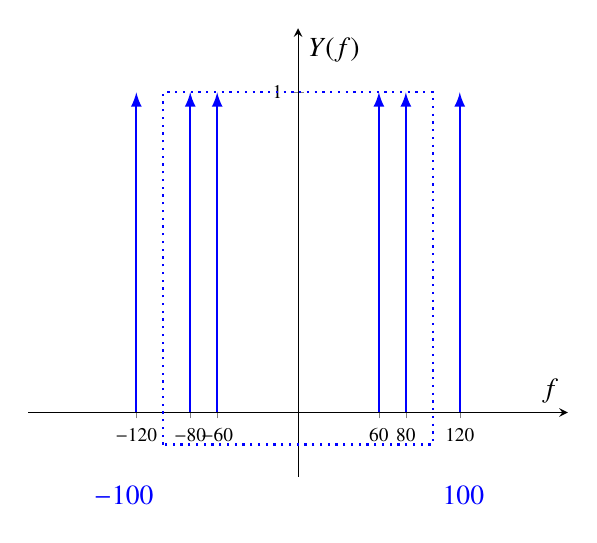
\begin{tikzpicture}
\begin{axis}[
    axis lines=middle,
    xlabel=$f$,
    ylabel=$Y(f)$,
    ymax=1,
    ymin=0,
    xmin=-200,
    xmax=200,
    xtick={ -120, -80, -60, 60, 80, 120},
    ytick={0,1},
    yticklabels={0,1},
    ticklabel style={font=\scriptsize},
    enlargelimits={abs=0.2},
    clip=false
]
% One-sided arrows
\draw[->, >=latex, blue, thick] (axis cs: -120, 0) -- (axis cs: -120, 1);
\draw[->, >=latex, blue, thick] (axis cs: -80, 0) -- (axis cs: -80, 1);
\draw[->, >=latex, blue, thick] (axis cs: -60, 0) -- (axis cs: -60, 1);
\draw[->, >=latex, blue, thick] (axis cs: 60, 0) -- (axis cs: 60, 1);
\draw[->, >=latex, blue, thick] (axis cs: 80, 0) -- (axis cs: 80, 1);
\draw[->, >=latex, blue, thick] (axis cs: 120, 0) -- (axis cs: 120, 1);
% Dotted box
\draw[blue, dotted, thick] (axis cs: -100, -0.1) rectangle (axis cs: 100, 1);
\node[blue, below right] at (axis cs: 100, -0.2) {$100$};
\node[blue, below left] at (axis cs: -100, -0.2) {$-100$};
\end{axis}
\end{tikzpicture}

	\caption{delta function of sampled and filtered signal }
\end{figure}
	from table $f_c = 100Hz$ \\
	LPF output : $60Hz$ , $80Hz$\\
	Maximum Frequency present in the filtered signal is $80Hz$.
	
	
	

\pagebreak
\item In the circuit shown, the input voltage $V_{in} = 100mV$. The switch and the opamp are ideal. At time $t=0$, the intial charge stored in the $10nF$ capacitor is $1nC$, with the polarity as indicated in the figure. The switch $S$ is controlled using a $1KHz$ square-wave voltage signal $V_s$ as shown. Whenever $V_s$ is `High', $S$ is in position $`1$' and when $V_s$ is `Low', $S$ is in position `$2$'.\\
At $t = 20ms$, the magnitude of the voltage $V_o$ will be  \\  
\begin{figure}[ht]
  \centering
    \resizebox{0.55\columnwidth}{!}{\begin{circuitikz}[american]
    \draw (0,0) node[op amp] (opamp) {};
    \draw (opamp.+) to [short] ++(-1,0) coordinate (leftLine) -- ++(0,-1) node[ground] {};
    \draw (opamp.-) to [short] ++(-1,0) to [short] ++(0,2) to [C, l_={$-$\hspace{1pt}$10nF$\hspace{1pt}$+$}] ++(2,0) to [short] ++(2,0) to [short] ++(0,-2.5);
    \draw (opamp.out) to [short] ++(1.5,0) node[right] {$V_o$};
    \draw (opamp.-) to [short] ++(-2.3,0);
    \draw[thick] ($(opamp.-) + (-2.7,0)$) -- ++(-2.3,0) node[left] (Vin) {$V_{in}$};
    \draw[dotted] ($(Vin.west) + (-1,-0.15)$) -- ($(Vin.west) + (-1,-0.85)$);
    \draw[thick] ($(Vin.west) + (-1,-0.4)$) ++(0,0.15) -- ++(0.5,0) -- ++(0,-0.5)-- ++(0.5,0)  -- ++(0,0.5) -- ++(0.5,0) -- ++(0,-0.5) -- ++(0.5,0) -- ++(0,0.5)  -- ++(0.5,0) -- ++(0,-0.5) -- ++(0.5,0);
    \node[font=\scriptsize] at ($(Vin.west) + (-1.5,-0.15)$) {High};
    \node[font=\scriptsize] at ($(Vin.west) + (-1.5,-0.65)$) {Low};
    \node[font=\scriptsize] at ($(Vin.west) + (-1,-0.85)$) {$t=0$};
    \draw[dotted] ($(Vin.west) + (3.1,0)$) -- ++(0.2,-0.3);
    \draw[dotted] ($(Vin.west) + (3.5,0)$) -- ++(-0.2,-0.3);
    \node[font=\scriptsize] at ($(Vin.west) + (3.3,0) + (0,0.5)$) {S};
    \draw[thick] ($(Vin.west) + (3.3,-0.3)$) -- ++(0,-1) to [C, l=$1nF$] ++(0,-1) node[ground] {};
    \node[font=\scriptsize] at ($(Vin.west) + (3.1,0.15)$) {1};
    \node[font=\scriptsize] at ($(Vin.west) + (3.5,0.15)$) {2};
\end{circuitikz}


}
\end{figure}
\hfill{(GATE IN 2023)}\\
\solution
\pagebreak

\item The value of parameters of the circuit shown in the figure are $R_1=2\ohm$,$R_2=2\ohm$,$R_3=3\ohm$,$L=10 mH$,$C=100\mu F$. For time \(t<0\), the circuit is at steady state with the switch $ 'K'$ in closed condition. If the switch is opened at $t=0$, the value of the voltage across the inductor \brak{V_L}
 at $t=0^{+}$ in Volts is \rule{2cm}{0.4pt} (Round off to 1 decimal place).
\begin{circuitikz}
    \draw (0,0) to [R, R=$R_3$] (0,2);
    \draw (0,3) to [switch, o-o, name=$K$] (0,2);
    \draw (0,3)-- (0,4);
    \draw (0,4) -- (4,4);
    \draw (3,0) to [american current source, l=$10\,\text{A,}\text{DC}$] (3,4);
    \draw (4,4) to (4,5) to (5,5) to[R, l=$R_1$] (6,5);
    \draw (6,5) to(7,5) to[L, l=$L$] (8,5) to (9,5);
    \draw (4,4)to (4,3)to (5,3) to[R, l=$R_2$] (6,3);
    \draw (6,3)to (7,3) to [C, l=$C$] (8,3) to(9,3);
    \draw (9,5) --(9,3);
    \draw (9,4) -- (10,4);
    \draw (10,4)-- (10,0);
    \draw(10,0)--(0,0);
\end{circuitikz} \hfill (GATE 2023 EE 29Q)
\solution
\pagebreak

\item The op amps in the circuit are ideal. The input signals are $V_{S1} = 3 + 0.10 \sin(300t), \text{V}$ and $V_{S2} = -2 + 0.11 \sin(300t)\, \text{V}$. The average value of the voltage $V_0$ is \underline{\hspace{1cm}} volts (rounded off to two decimal places).
\begin{figure}[ht]
\centering
\resizebox{0.55\columnwidth}{!}{\input{2023/IN/59/figs/gate.circuit.tex}}
\end{figure}
\hfill{(GATE IN 2023)}
\solution
\iffalse
\let\negmedspace\undefined
\let\negthickspace\undefined
\documentclass[journal,12pt,twocolumn]{IEEEtran}
\usepackage{cite}
\usepackage{amsmath,amssymb,amsfonts,amsthm}
\usepackage{algorithmic}
\usepackage{graphicx}
\usepackage{textcomp}
\usepackage{xcolor}
\usepackage{txfonts}
\usepackage{listings}
\usepackage{enumitem}
\usepackage{mathtools}
\usepackage{gensymb}
\usepackage{comment}
\usepackage[breaklinks=true]{hyperref}
\usepackage{tkz-euclide}
\usepackage{listings}
\usepackage{gvv}
\def\inputGnumericTable{}
\usepackage[latin1]{inputenc}
\usepackage{color}
\usepackage{array}
\usepackage{longtable}
\usepackage{calc}
\usepackage{multirow}
\usepackage{hhline}
\usepackage{ifthen}
\usepackage{lscape}
\usepackage{circuitikz}

\newtheorem{theorem}{Theorem}[section]
\newtheorem{problem}{Problem}
\newtheorem{proposition}{Proposition}[section]
\newtheorem{lemma}{Lemma}[section]
\newtheorem{corollary}[theorem]{Corollary}
\newtheorem{example}{Example}[section]
\newtheorem{definition}[problem]{Definition}
\newcommand{\BEQA}{\begin{eqnarray}}
\newcommand{\EEQA}{\end{eqnarray}}
\newcommand{\define}{\stackrel{\triangle}{=}}
\theoremstyle{remark}
\newtheorem{rem}{Remark}
\begin{document}

\bibliographystyle{IEEEtran}
\vspace{3cm}

\title{Gate 2023- Instrumentation Engineering}
\author{EE23BTECH11037 - M Esha$^{*}$% <-this % stops a space
}
\maketitle
\newpage
\bigskip

\renewcommand{\thefigure}{\theenumi}
\renewcommand{\thetable}{\theenumi}

\vspace{3cm}
\textbf{Question 59:} 
The op amps in the circuit are ideal. The input signals are $V_{S1} = 3 + 0.10 \sin(300t), \text{V}$ and $V_{S2} = -2 + 0.11 \sin(300t)\, \text{V}$. The average value of the voltage $V_0$ is \underline{\hspace{1cm}} volts (rounded off to two decimal places).

\begin{figure}[ht]
\centering
\resizebox{0.55\columnwidth}{!}{\input{2023/IN/59/figs/gate.circuit.tex}}
\end{figure}
\hfill{(GATE IN 2023)}\\
\solution
\fi
\begin{table}[h!]
  \centering
  \begin{tabular}{|c|c|c|}
  \hline
  \textbf{Variable} & \textbf{Value} & \textbf{Description} \\
  \hline
  $V_{s1}$ & $3 + 0.10 \sin(300t)$ & \multirow{2}{*}{Input voltages} \\
  \cline{1-2}
  $V_{s2}$ & $-2 + 0.11 \sin(300t)$ & \\
  \cline{1-3}
  $R$ & & Resistances of the resistors \\
  \cline{1-3}
  $V_o$ & & Output voltage \\
  \cline{1-3}
  $V_1$ & & Output voltage of $V_{s1}$ opamp \\
  \cline{1-3}
  $V_2$ & & Output voltage of $V_{s2}$ opamp \\
  \hline
\end{tabular}

  \caption{Input Parameters}
    \label{tab:tableeshaa1}
\end{table}\\
the current does not flow through op-amp. voltage drop by each R
\begin{align}
&= V_{s1}-V_{s2}
\end{align}
by KVL,
\begin{align}
V_{s2}-V_2&=V_{s1}-V_{s2}\\
V_2&=2V_{s2}-V_{s1}\\
V_1-V_{s1}&=V_{s1}-V_{s2}\\
V_1&= 2V_{s1}-V_{s2}\\
V_o&= \frac{V_1+V_2}{2}\\
&=\frac{V_{s1}+V_{s2}}{2}\\
&=\frac{3+0.10\sin(300t)+{-2}+0.11\sin(300t)}{2}\\
&=0.5+ \frac{0.21\sin(300t)}{2}\\
V_{avg}&=\frac{1}{T} \int_{0}^{T} V(t) \,dt\\
&=\frac{300}{2\pi} \int_{0}^{\frac{2\pi}{300}} \left(0.5 + \frac{0.21 \sin(300t)}{2}\right) \, dt\\
&=0.5
\end{align}
\begin{figure}[b]
    \centering
    \includegraphics[width=\columnwidth]{2023/IN/59/figs/59fig.png}
    \caption{line plot }
    \label{fig:eshaa1}
\end{figure}
%\end{document}


\pagebreak

\end{enumerate}
